\section{Results}
To evaluate our pipeline synthesis tool, we write a 2-stage, 3-stage,
4-stage, and 5-stage pipeline specification for a single cycle CPU
datapath. We present CPI results to show that our synthesis tool is
effective in improving performance. We also push our auto-generated
pipeline through Design Compiler synthesis tool using TSMC's 45nm CMOS
library and compare the post-synthesis results to hand-coded 2-stage,
3-stage, 4-stage, and 5-stage pipelines.

\subsection{Sodor}
Sodor is a set of simple processors written in Chisel. We use Sodor's
1-stage processor for the datapath specification. In order to work
with our tool, we modify the 1stage to use {\tt TransacationalMem}
instead of {\tt Mem} and wrapped the instruction and data cache with
our variable latency interface. Sodor also provides 2 and 5-stage
in-order processor that we use to compare against our auto-generated 2
and 5-stage processor. We had to write a 3-stage and 4-stage processor
ourselves. The hand-coded 2-stage has speculation on the PC
register. The 3, 4, and 5-stage processors make use of speculation on
the PC register and bypassing to forward results from the ALU and the
data cache.

\subsection{Comparison}
\begin{figure*}
\centering
  \begin{subfigure}[t]{0.47\textwidth}
  \centering
  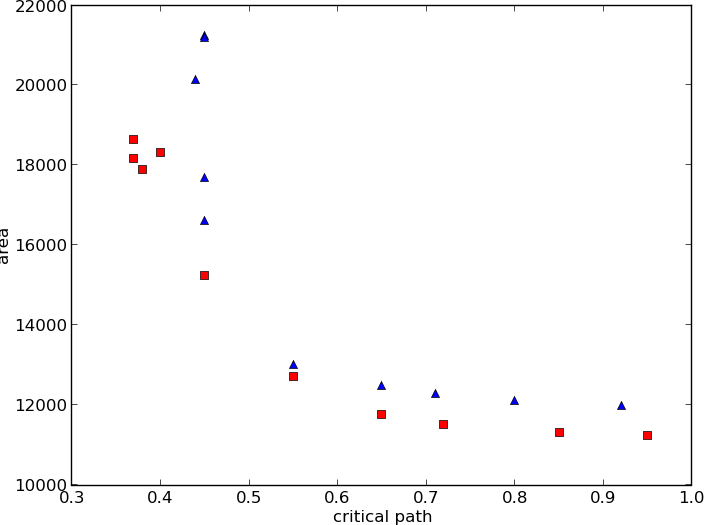
\includegraphics[width=\textwidth]{figures/2stage.png}
  \caption{2-stage}
  \label{fig:2stage}
  \end{subfigure}
  \hfill
  \begin{subfigure}[t]{0.47\textwidth}
  \centering
  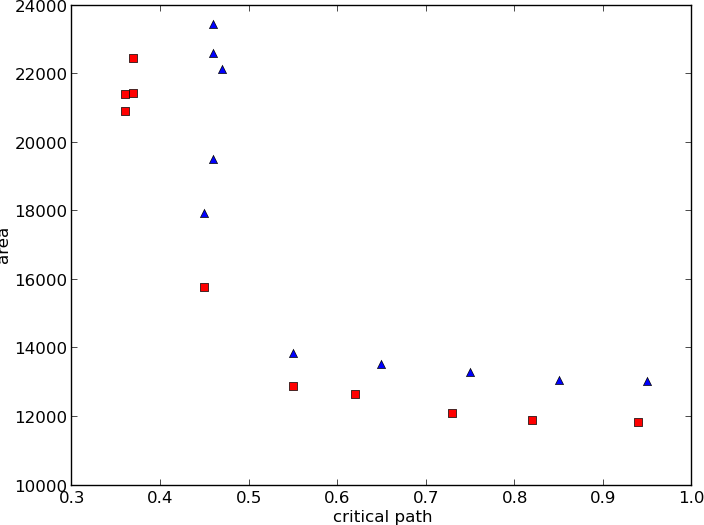
\includegraphics[width=\textwidth]{figures/3stage.png}
  \caption{3-stage}
  \label{fig:3stage}
  \end{subfigure}
  \hfill
  \begin{subfigure}[t]{0.47\textwidth}
  \centering
  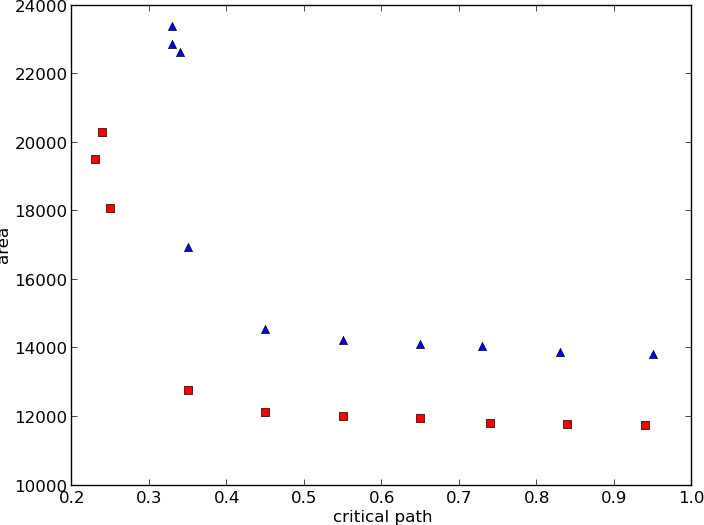
\includegraphics[width=\textwidth]{figures/4stage.png}
  \caption{4-stage}
  \label{fig:4stage}
  \end{subfigure}
  \hfill
  \begin{subfigure}[t]{0.47\textwidth}
  \centering
  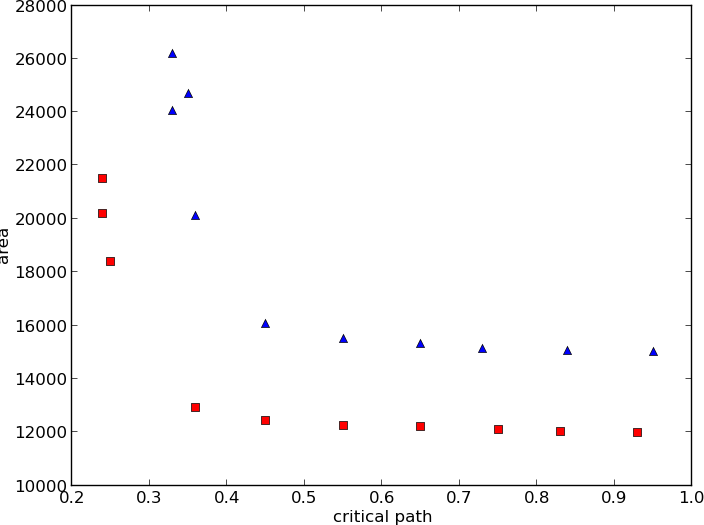
\includegraphics[width=\textwidth]{figures/5stage.png}
  \caption{5-stage}
  \label{fig:5stage}
  \end{subfigure}
\end{figure*}
